\documentclass[parskip=half,notes,cadrem,toolver]{iisvlsi}
%
%
%
% Package loading required for *this* document.
\usepackage[utf8]{inputenc}
\usepackage[english]{babel}
\usepackage{lipsum}
\usepackage{tabularx}
\usepackage{caption}
\usepackage{subcaption}
\usepackage{textcomp}
\usepackage{siunitx}
\usepackage{hyperref}
\usepackage{dirtree}
\usepackage{graphicx}
\usepackage{float}
\usepackage{listings} 
\usepackage[acronym]{glossaries}
\usepackage{datetime} 
\usepackage{textgreek}
\usepackage[toc]{appendix}
\usepackage{xurl} 

\newacronym{mcu}{MCU}{Microcontroller}
\newacronym{gpio}{GPIO}{General Purpose Input/Output}
\newacronym{uart}{UART}{Universal Asynchronous Receiver Transmitter}
\newacronym{cmsis}{CMSIS}{Cortex Microcontroller Software Interface Standard}
\newacronym{dsp}{DSP}{Digital Signal Processor}
\newacronym{ide}{IDE}{Integrated Development Environment}
\newacronym{rtos}{RTOS}{Real-Time Operating System}
\newacronym{hal}{HAL}{Hardware Abstraction Layer}
\newacronym{fft}{FFT}{Fast Fourier Transformation}
\newacronym{dct}{DCT}{Discrete Cosine Transform}
\newacronym{simd}{SIMD}{Single Instruction Multiple Data}
\newacronym{mac}{MAC}{Multiply-Accumulate}
\newacronym{pdm}{PDM}{Pulse-Density Modulation}
\newacronym{dfsdm}{DFSDM}{Digital Filter for Sigma-Delta Modulator}
\newacronym{ml}{ML}{Machine Learning}
\newacronym{svm}{SVM}{Support Vector Machine}
\newacronym{nn}{NN}{Neural Network}
\newacronym{ann}{ANN}{Artificial Neural Network}
\newacronym{mlp}{MLP}{Multi-Layer Perceptron}
\newacronym{sgd}{SGD}{Stochastic Gradient Descent}

%
%
%
% Titlepage settings.
\exdesc{Exercise 3}
\extitle{Model training and evaluation: \\ an introduction to scikit-learn \& Keras/PyTorch}
\lecturer{Michele Magno, PhD\\ 
Viviane Potocnik \\
Marco Giordano \\
Pietro Bonazzi
}
\course{Machine Learning on Microcontrollers}
\coursenr{227-0155-00L}
\docvers{}
\lastchange{}
\newdate{date}{02}{10}{2024}
\date{\displaydate{date}}
%
%


\lstset{
    language=Python,
    basicstyle=\ttfamily\footnotesize,
    keywordstyle=\color{blue},
    commentstyle=\color{green},
    stringstyle=\color{red},
    numbers=left,
    numberstyle=\tiny\color{gray},
    frame=single,
    breaklines=true
}
%
\begin{document}

%
% Do not change the following line, because it is used in order to derive SVN-specific information from the present file.
\svnidlong
{$HeadURL: svn://iis-svn.ee.ethz.ch/mbgh/docs/latex/classes/iisvlsi/iisvlsi_sample.tex $}
{$LastChangedDate: 2012-02-23 13:48:26 +0100 (Thu, 23 Feb 2012) $}
{$LastChangedRevision: 56 $}
{$LastChangedBy: mbgh $}
\svnid{$Id: iisvlsi_sample.tex 56 2012-02-23 12:48:26Z mbgh $}
%
%
% Generate the title page with the previously defined settings.
\maketitle
%

%\printglossaries
%
\section{Introduction}
In this lab session you will learn the basics of \gls{ml} and have a practical experience on how to use the most common \gls{ml} tools to solve classification tasks.

If you don't have any experience with \gls{ml} or you want to review what you already know, you can read through this section to get the core ideas. Otherwise, you can jump directly to section~\ref{sec:prep} for the exercises.

\subsection{Basics of Machine Learning}

\gls{ml} is defined as a set of methods that can automatically detect patterns in data, and then use the uncovered patterns to predict future data, or to perform other kinds of decision making under uncertainty (ref. K. P. Murphy, \textit{Machine Learning A Probabilistic Perspective}).

There are different kinds of \gls{ml} problems, such as:
\begin{itemize}
    \item Classification: the goal is to learn an indicator function. For example, given a dataset containing pictures of cats and dogs, you want your model to learn how to separate cats from dogs, i.e. given new pictures of cats or dogs, the model should be able to correctly tell if it's a picture of a cat or a picture of a dog.
    \item Regression: the goal is to learn a real-valued function. For example, one wants to predict the height of a person knowing his/her shoe size or predict how the sales of passenger vehicles in India will be next year.
    \item Dimension reduction: the goal is to learn a linear or non-linear projection of your dataset. One example is the so-called maximally informative dimensions technique, which is a dimensionality reduction technique used in neuroscience to project a neural stimulus onto a low-dimensional subspace so that as much information as possible about the stimulus is preserved in the neural response.
    \item Data compression: the goal is to learn an encoding for efficient representation, for example image or audio compression. Data compression can be either lossy or lossless (e.g. dimensionality reduction is a form of lossy compression).
\end{itemize}

There are four types of learning:
\begin{itemize}
    \item Supervised learning: learn a function that maps an input to an output based on example input-output pairs (labels given). Examples of supervised learning algorithms: Decision Trees, Nearest Neighbor, Naïve Bayes, Linear Regression, SVM, etc.
    \item Unsupervised learning: learn from test data that has not been labeled, classified or categorized (no labels). Examples: K-means clustering, association rules, density estimation, PCA, etc.
    \item Semi-supervised learning: make use of unlabeled data for training – typically a small amount of labeled data with a large amount of unlabeled data
    \item Reinforcement learning: take actions in an environment so as to maximize some notion of cumulative reward
\end{itemize}

In this course we will mostly be focusing on classification or regression tasks using supervised learning techniques.

\subsection{General Workflow}
Figure~\ref{fig:workflow} shows the general \gls{ml} workflow for a supervised learning case.

\begin{figure}[H]
    \begin{center}
        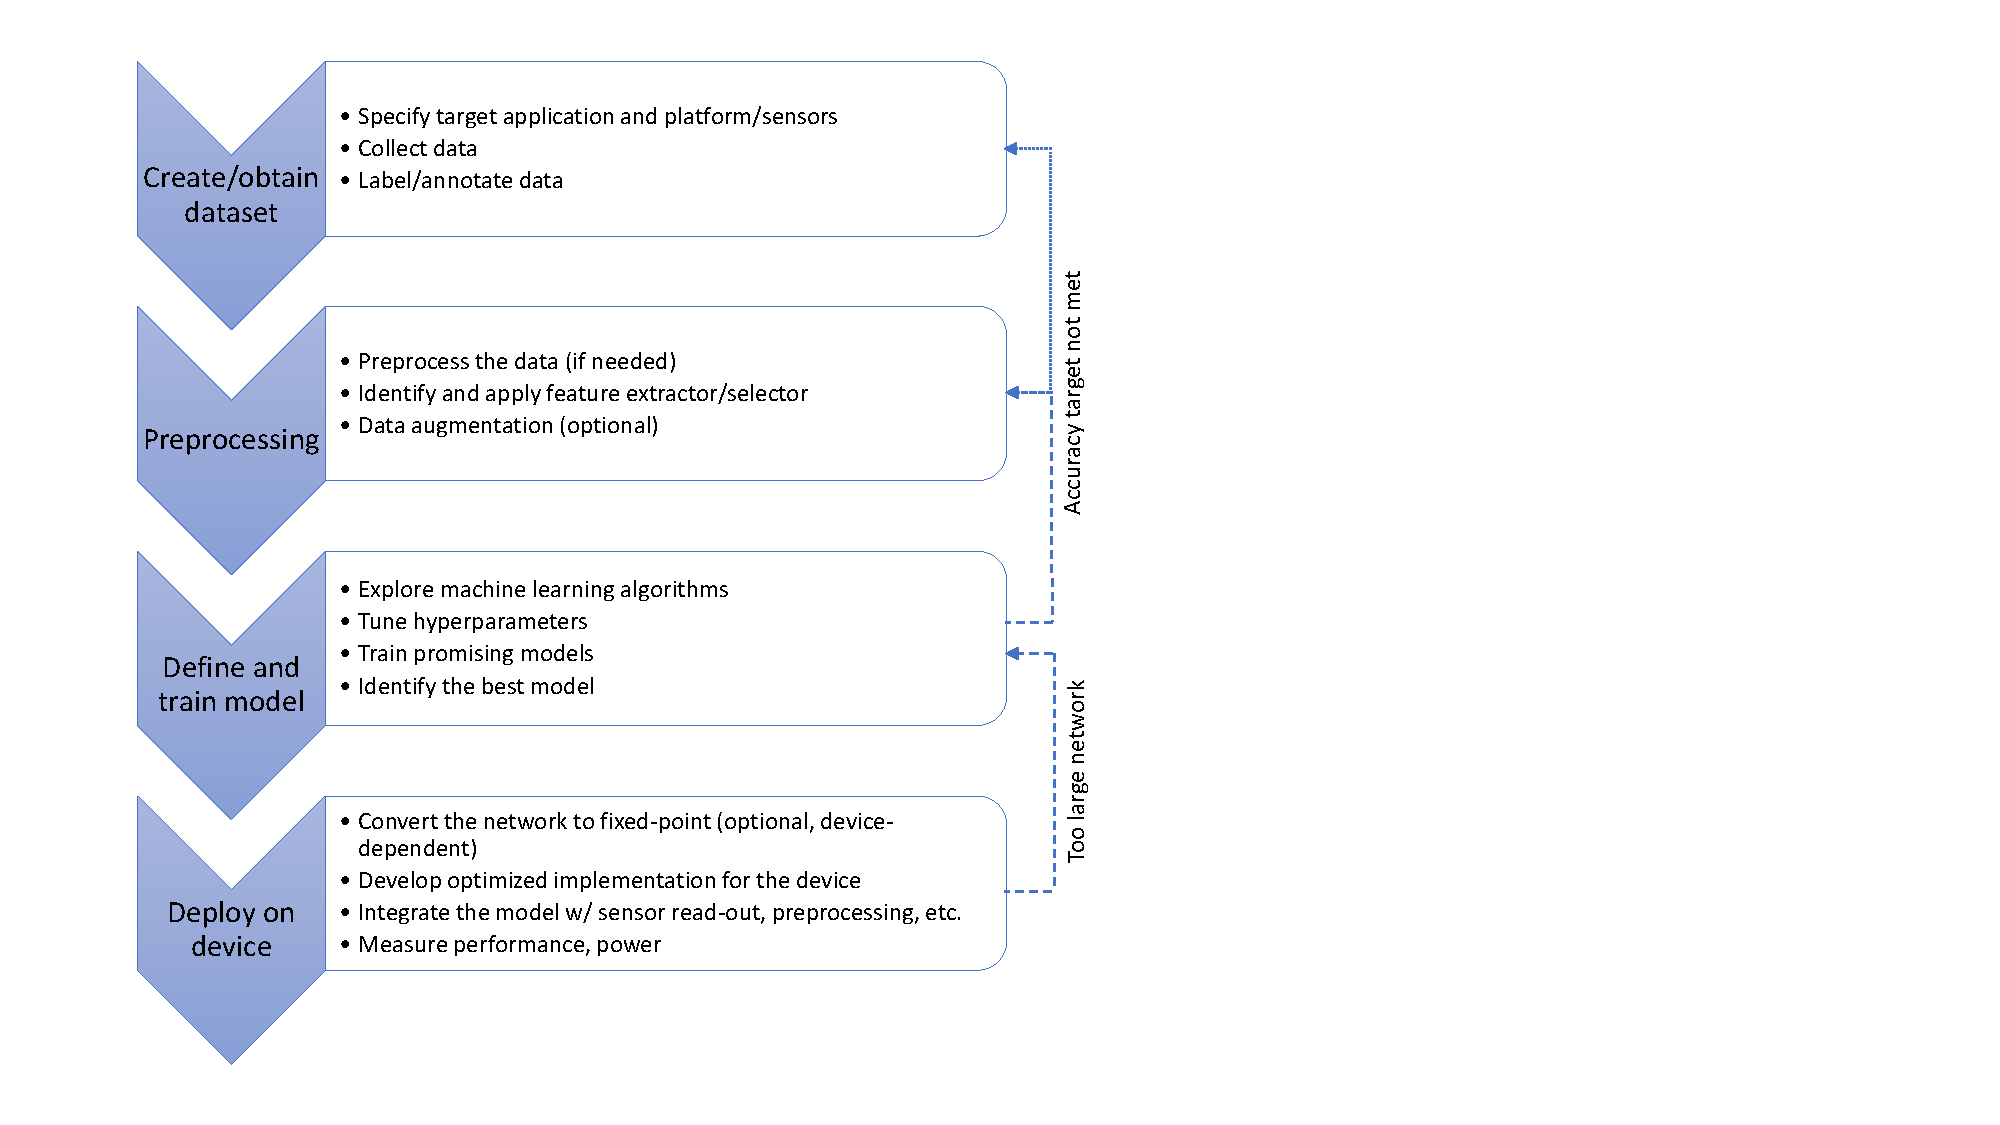
\includegraphics[trim={1.2cm, 0.8cm, 15cm, 1cm}, clip=true, width=0.6\linewidth]{figures/workflow-lab.pdf}
        \caption{General \gls{ml} workflow.}
        \label{fig:workflow}
    \end{center}
\end{figure}

After identifying your target application, you first collect the dataset and label it if it's not already available, then apply preprocessing steps, if needed, to clear the data and enhance the signal-to-noise ratio followed by feature extract and/or selection. Afterwards, you split the dataset and start the training process. The dataset is divided into:
\begin{itemize}
    \item Training set: used for learning the function (fit the parameters, e.g. weights, of for example a classifier) which maps the input to the output.
    \item Validation set: used for validating the model, i.e. identify the model and tune the hyperparameters (i.e. the architecture) of a classifier. It also helps to avoid overfitting.
    \item Test set: independent from the other sets and used for testing the final trained model. If a model which fits to the training dataset also fits the test dataset well, minimal overfitting has taken place.
\end{itemize}

It is common to find \gls{ml} applications where the training set and the validation set are merged into one single set (e.g. using cross-validation when the dataset is small). Sometimes the validation set is called test set, and the final model is directly tested on real-world data during application.

\subsection{Underfitting and Overfitting}
One of the key points in \gls{ml} is the problem of underfitting/overfitting. When you train a model, you want your trained model to be able to generalize, i.e. the model should be able to give sensible outputs to sets of input that it has never seen before. Based on this idea, the term underfitting and overfitting refer to deficiencies in the model’s performance to predict on unseen data.

Overfitting, or sometimes called overtraining, happens when a statistical model contains more parameters than the amount of data available for training. In other words, the model fits too closely or exactly to a particular set of data, such that some of the residual variation (i.e. the noise) is also extracted as if that variation represented underlying model structure. Overfitted model may therefore fail to fit additional data or predict future observations reliably. An illustrative example of overfitting on linear regression is shown in Figure~\ref{fig:overfitting}.

Contrarily, underfitting, or undertraining, occurs when the trained model cannot appropriately capture the underlying structure of the data (see Figure~\ref{fig:underfitting}). It happens when the model lacks some parameters or terms that would be necessary for a correctly specified model. For example, it occurs when fitting a linear model to non-linear data. Such a model will not be able to predict the non-linear behaviour of the data.

Finally, Figure~\ref{fig:good} shows the desired predictive model in an example of linear regression.

\begin{figure}[H]
     \centering
     \begin{subfigure}[b]{0.3\textwidth}
         \centering
         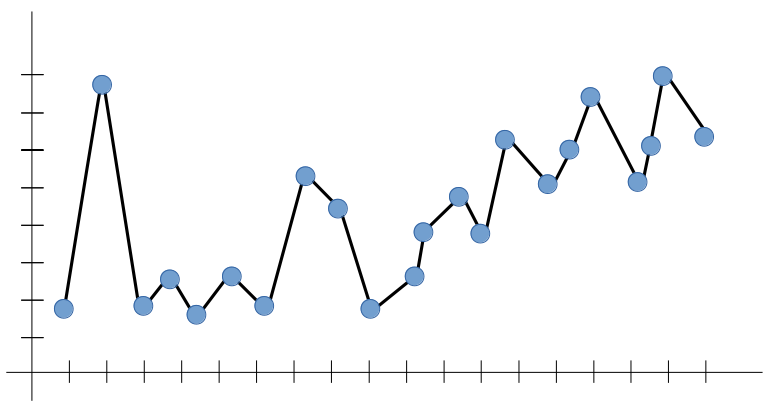
\includegraphics[width=\textwidth]{figures/overfitting.png}
         \caption{Overfitting.}
         \label{fig:overfitting}
     \end{subfigure}
     \hfill
     \begin{subfigure}[b]{0.3\textwidth}
         \centering
         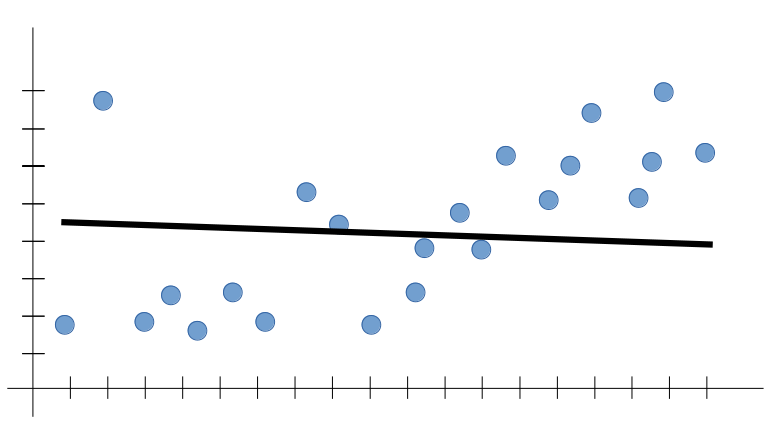
\includegraphics[width=\textwidth]{figures/underfitting.png}
         \caption{Underfitting.}
         \label{fig:underfitting}
     \end{subfigure}
     \hfill
     \begin{subfigure}[b]{0.3\textwidth}
         \centering
         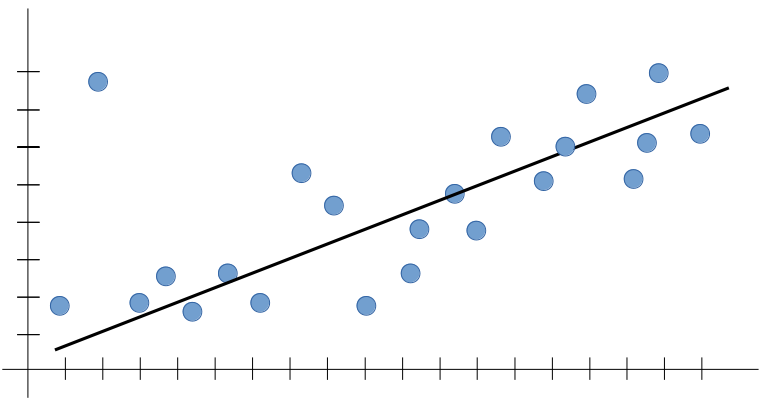
\includegraphics[width=\textwidth]{figures/good.png}
         \caption{Desired model.}
         \label{fig:good}
     \end{subfigure}
        \caption{Illustrative example of overfitting and underfitting based on linear regression problem.}
        \label{fig:under-over-fitting}
\end{figure}

\ifx
\section{Examples of ML algorithms}
Here we provide a short description of two ML algorithms: Decision Trees (DTs) and Support Vector Machines (SVMs).

\subsection{Decision Trees}
Decision tree learning is a supervised learning method used in ML. It uses tree-like structure where each branch represents an observation about a feature of the input data, and each leaf node represents a class label, i.e. target value. Figure~\ref{fig:dt} shows an example of DT. These models are easy to implement (if-then constructs) and have low memory requirement and low complexity.

\subsection{Support Vector Machines}
TODO
\fi

\section{Introduction to Artificial Neural Networks}

\glspl{ann} are computing systems inspired by biology, more specifically the brain. The nervous system of most known beings is made up of many neurons, shown in Figure \ref{fig:neuron}, connected together in different ways. As a reference, a neuron may decide to 'fire', or transmit a signal along the axon to the synaptic terminals, based on the input signals at the dendrites. Connecting many millions of these together allows processing of information from vague inputs to valuable, more refined information.

An \gls{ann} attempts to emulate this, combining inputs in different ways and deciding whether or not to activate, thereby processing the given information, as shown in Figure~\ref{fig:ann_1}. Inputs, which may go to many different neurons, are each multiplied by a weight, computed during training. The sum of all these weighted inputs determines if the neuron 'fires' or not. Connecting these neurons to many layers allows similar processes as in biology, processing signals to valuable information.

\begin{figure}[H]
\centering
    \begin{subfigure}[t]{0.45\linewidth}
        \centering
        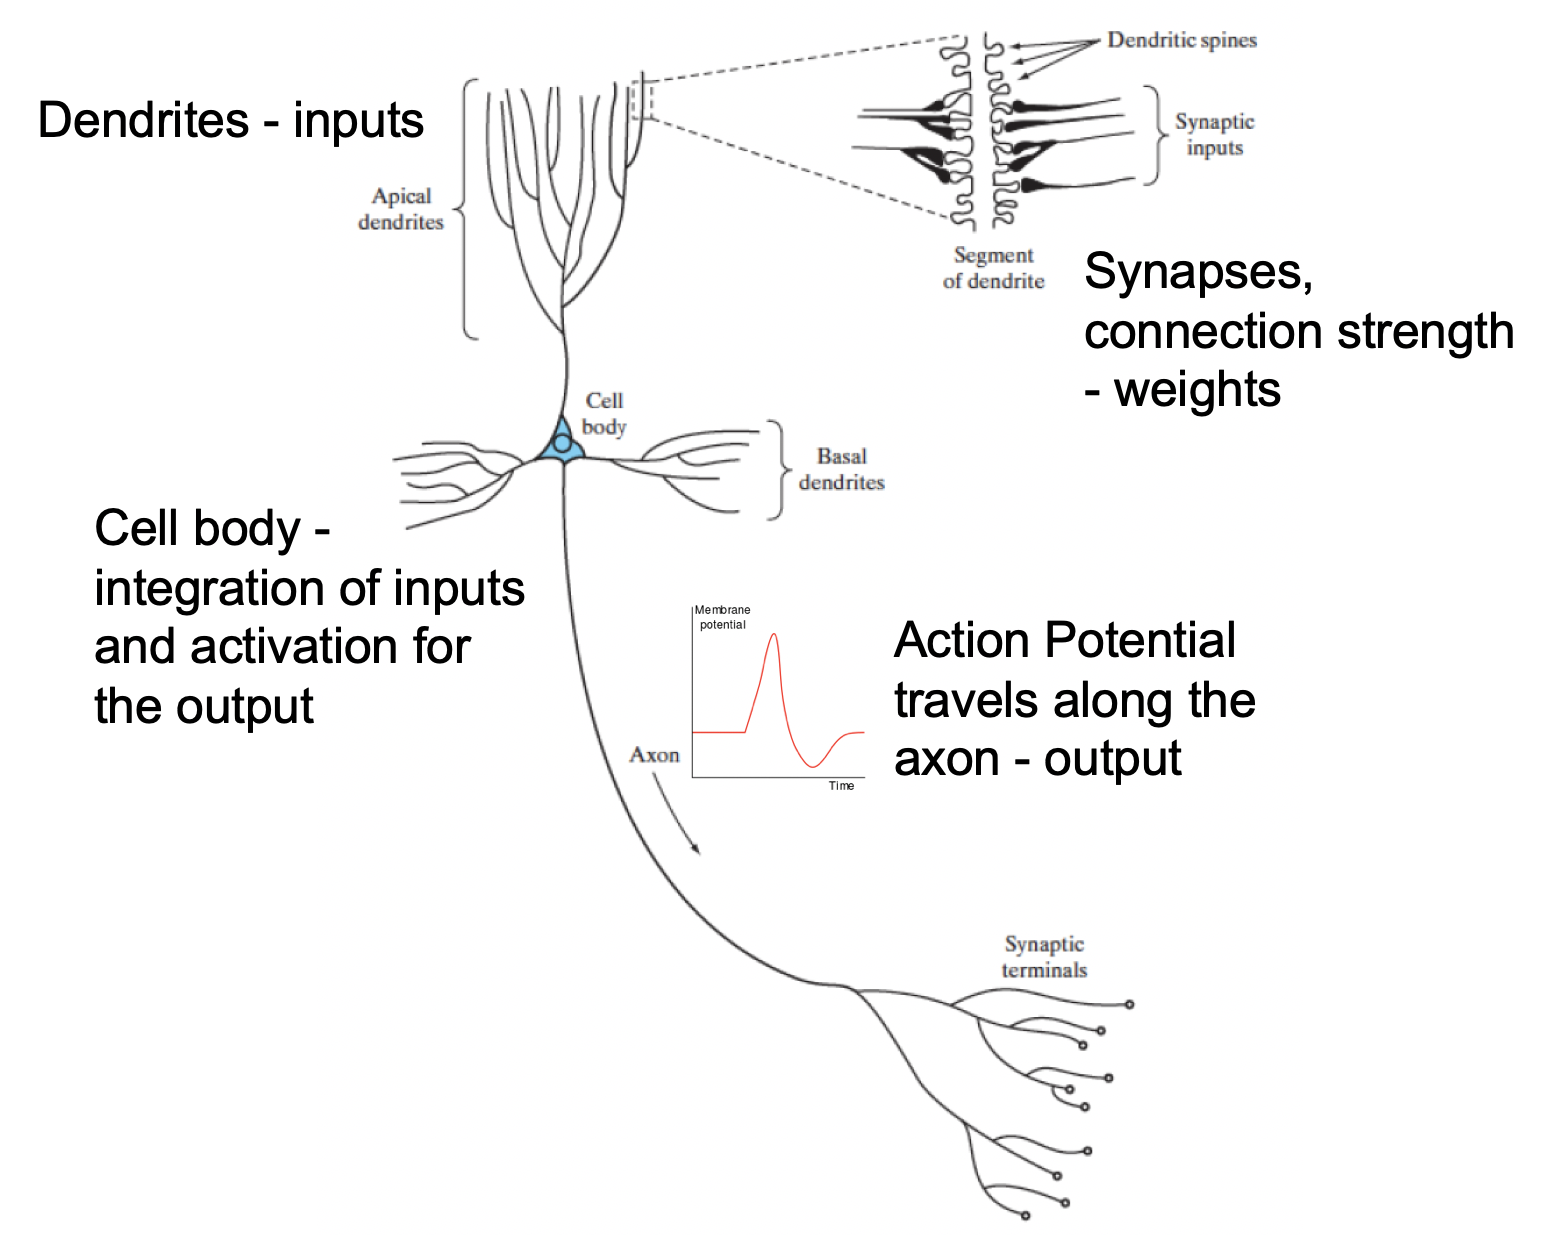
\includegraphics[width=\textwidth]{figures/Neuron.png}
        \caption{}
        \label{fig:neuron}
    \end{subfigure}
    \begin{subfigure}[t]{0.45\linewidth}
        \centering
        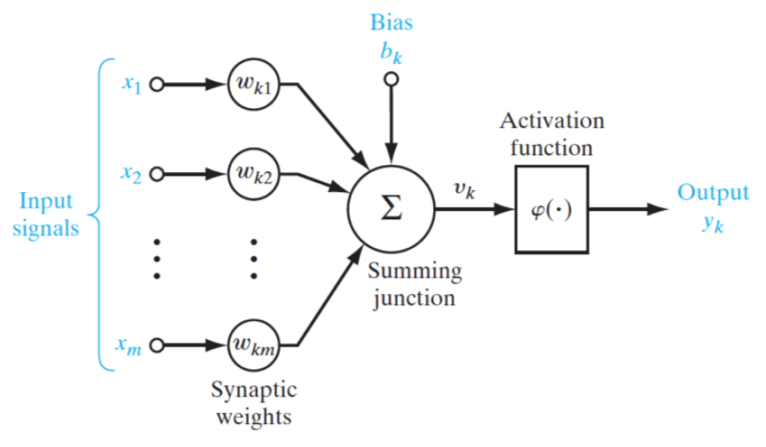
\includegraphics[width=\textwidth]{figures/ANN_1.png}
        \caption{}
        \label{fig:ann_1}
    \end{subfigure}
    \caption{Illustrations of biological neuron (a) and artificial neuron (b).}
    \label{fig:biological_artificial_nn}
\end{figure}


There are many ways neurons can be connected to each other, however the overall architecture is similar. Initially, the input data is transmitted through an input layer, which acts as an initial processor for the given data, often expanding the data to allow more detailed computations. Layers usually take many inputs, often sharing these with other neurons, and process these to produce one output. Structuring these in layers allows for sequential computation, taking signals from one layer and feeding them into the next. After the initial input layer, the signals are usually forwarded to many hidden layers, where the size and function may vary. Ultimately a final output layer is used to determine the result of the computation. 

\begin{figure}[H]
%\centering
    \begin{subfigure}[t]{0.33\linewidth}
        \centering
        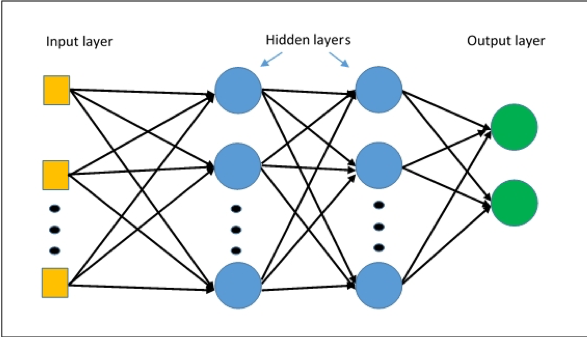
\includegraphics[width=\textwidth]{figures/ffnn.png}
        \caption{Feedforward \gls{nn}}
        \label{fig:ffnn}
    \end{subfigure}
    \begin{subfigure}[t]{0.33\linewidth}
        \centering
        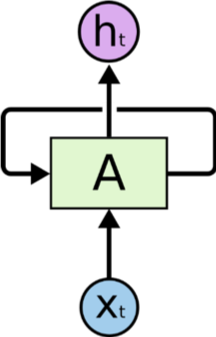
\includegraphics[width=0.4\textwidth]{figures/recnn.png}
        \caption{Recurrent \gls{nn}}
        \label{fig:recnn}
    \end{subfigure}
    \begin{subfigure}[t]{0.33\linewidth}
        \centering
        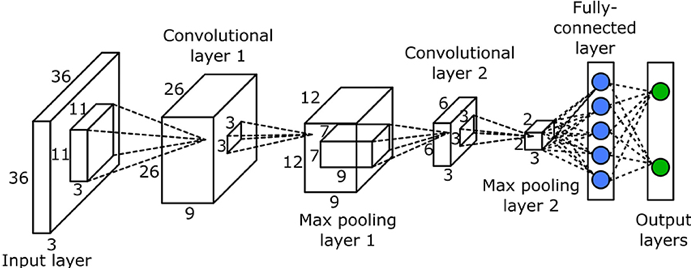
\includegraphics[width=\textwidth]{figures/cnn.png}
        \caption{Convolutional \gls{nn}}
        \label{fig:cnn}
    \end{subfigure}
    \caption{Commonly used types of artificial neural networks.}
    \label{fig:nns}
\end{figure}

There are different types of \glspl{nn}, mostly varying in the function of the hidden layers and the type of connections between neurons. Figure~\ref{fig:nns} demonstrates the most commonly used \glspl{nn}. Feedforward \glspl{nn} simply have neuron layers connected in a \emph{feedforward} way, i.e. the connections between the nodes do not form a cycle. Recurrent \glspl{nn} can use their internal state (memory) to process sequences of inputs and the connections between the nodes form a directed graph along a temporal sequence. Finally, convolutional \glspl{nn} have convolution layers where convolutional filters are seen as neurons and are applied to the input data (1D signals, 2D images, or 3D volumes). 

These different types of networks come with different advantages, e.g. recurrent networks allow for learning with respect to spatial or temporal dependencies of a series of input feature vectors whereas convolutional networks are best at image processing. During this course we will be using mostly feedforward \glspl{nn} and convolutional \glspl{nn}.


\section{Feedforward NNs (Multi-layer perceptrons)}

\subsection{Structure}

A feedforward \gls{nn}, as the name suggest, is a neural network which only processes information in the forward direction, i.e. there are no cycles or feedback paths. \gls{mlp} falls in this category. The neurons, in this case also called perceptrons, are arranged in subsequent layers and connected in a feedforward manner from the input to the output. If every neuron in a precedent layer is connected to all the neurons in the following layer, then the layer is called dense or fully-connected layer, otherwise it is named sparsely-connected layer. 

\begin{figure}[t]
    \centering
    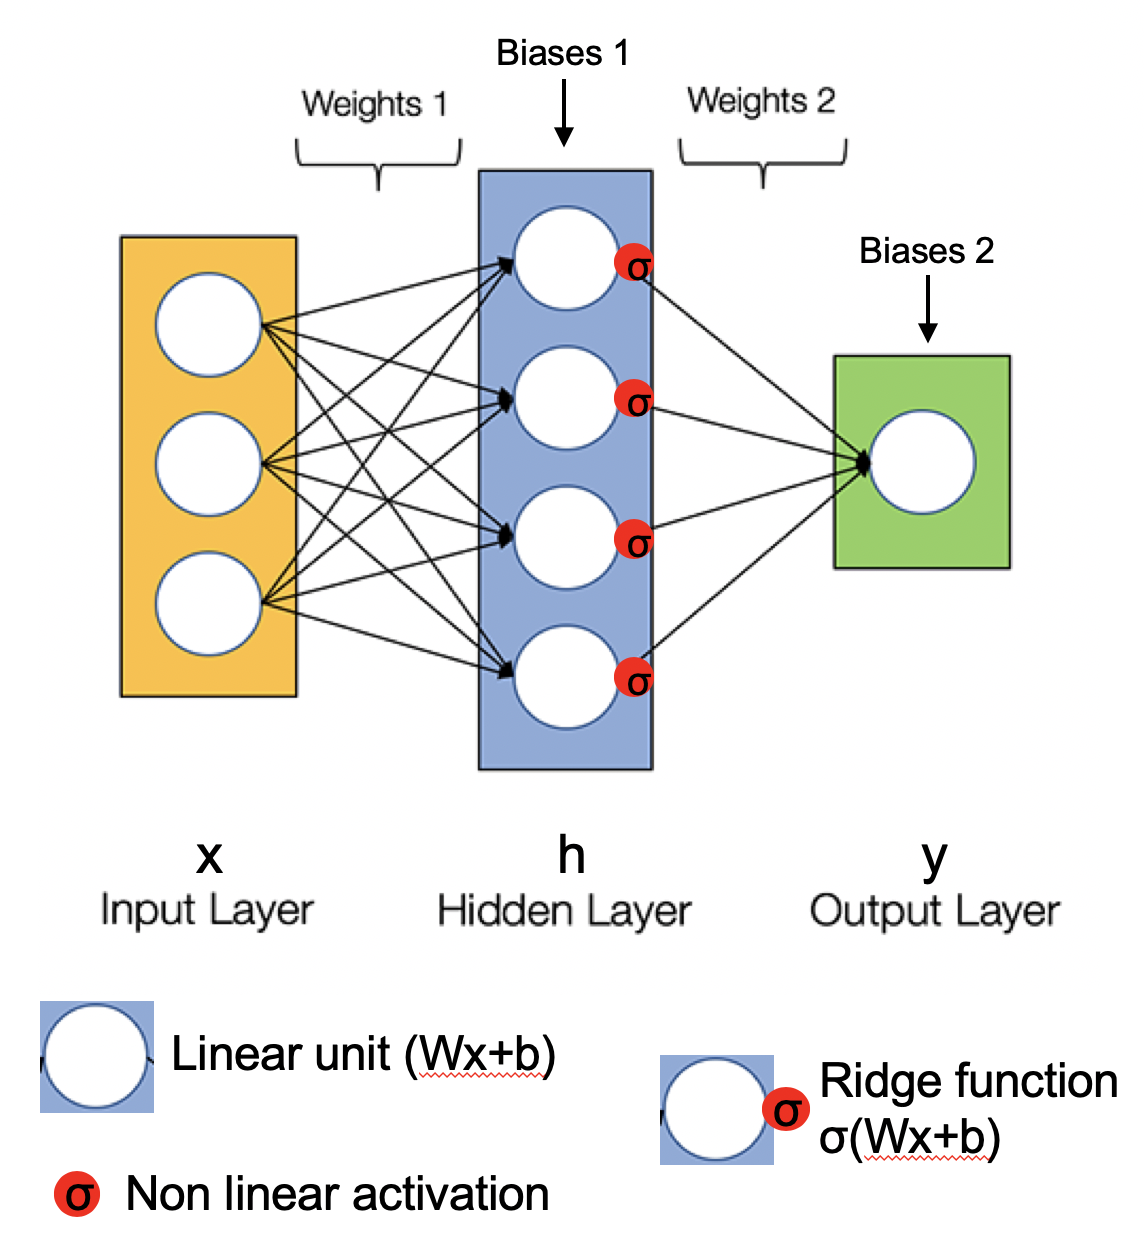
\includegraphics[width=0.5\textwidth]{figures/ANN_2.png}
    \caption{Structure of a feedforward neural network.}
    \label{fig:ann_2}
\end{figure}

Each perceptron can be modeled with a linear and a non-linear part, the linear part being a matrix multiplication of a learned weight matrix $W$ with the input vector $x$ and the addition of some bias vector $b$, i.e. $Wx+b$. The non-linear part comes with the activation function $\sigma$, turning the output of the neuron into $\sigma(Wx+b)$. Activation functions come in many styles, the most famous ones being ReLU, sigmoid and tanh.

\ifx
In the code snippet below a single hidden layer perceptron is declared:

\begin{lstlisting}
class NeuralNetwork:
    def __init__(self, x, y):
        self.input = x
        self.weights1 = np.random.rand(self.input.shape[1],4)
        self.weights2 = np.random.rand(4,1)
        self.y = y
        self.output = np.zeros(y.shape)
\end{lstlisting}
\fi

\subsection{Training a Neural Network}

For supervised learning, we are given large amounts of training data that each have an input $x$ and an output $y$. To train our network, we want to find $W$ and $b$ that solve following equation:

$$ \hat{y} = \sigma (W_2 \sigma (W_1 x + b_1) + b_2) $$

This however is a numerically hard task, since many matrix inversions are not well-conditioned and the inversion of the non-linear activation function might not even uniquely exist or be numerically unstable as well.

\subsection{Optimizers and Loss functions}

Due to the above mentioned difficulties, we do not actually ever invert any part of this equation and instead opt for stepwise optimization of our solution by using a method called backpropagation on a loss function. This so called loss function maps the output of our current solution and the correct output to some real number which represents the difference or error in output. Well-known loss functions are the quadratic error function or the cross-entropy. We then update the weights and biases of our network by backpropagating this loss with an optimizer.

The choice of loss function and optimizer is an art in and of itself, so some experience and experimentation can often lead to better results. 

To help you better understand this process, let's take a look at the most important optimizer, \gls{sgd} with momentum term. We formulate training as an optimization problem. Let $L_{i}$ be the loss function and $\omega$ the parameters of layer $i$ of the whole network:
$$ L(\omega) = \sum_{i} L_{i}(\omega) $$
$$\text{minimze } L(\omega)$$

The choice of optimizer dictates how we go about minimizing the loss function. The most important and standard optimizer is called \gls{sgd} and optimizes by simply updating $\omega$ in the direction of steepest descent.
The standard version would update $\omega$ by the following rule:
$$\omega := \omega - \eta \nabla L(\omega)$$
where we call $\eta$ the learning rate.

Since this form only takes into account gradient, we might end up in a local minimum, which might not be what we want. To solve this problem, we can add a momentum term, which allows us to "escape" a local minimum. The rule is then adapted as follows:

$$ \Delta\omega := \alpha\Delta\omega' - \eta\nabla L(\omega) $$
$$ \omega := \omega + \Delta\omega $$

Where $\omega'$ is the previous update of the weights. This leads to two parameters we can tune, learning rate $\eta$ and momentum term $\alpha$. Controlling these two parameters can be essential to end up with a well-working network.

There are some more abstractions that are used with the training process, like minibatching, rate decay and many more, the essential part however is understanding the way the loss function and the optimizer work. 

In the next example the quadratic error loss function is implemented and used with a \gls{sgd} optimizer without momentum term.

% TODO: maybe add caption to this?
\begin{lstlisting}
class NeuralNetwork:
    def __init__(self, x, y):
        self.input = x
        self.weights1 = np.random.rand(self.input.shape[1],4)
        self.weights2 = np.random.rand(4,1)
        self.y = y
        self.output = np.zeros(y.shape)
    
    def feedforward(self):
        self.layer1 = sigmoid(np.dot(self.input, self.weights1))
        self.output = sigmoid(np.dot(self.layer1, self.weights2))
        
    def backprop(self):
        # application of the chain rule to find derivative of the loss
        #   function with respect to weights2 and weights1
        d_weights2 = np.dot(self.layer1.T, (2*(self.y - self.output) *
            sigmoid_derivative(self.output)))
        d_weights1 = np.dot(self.input.T,  (np.dot(2*(self.y - self.output) * 
            sigmoid_derivative(self.output), self.weights2.T) * 
            sigmoid_derivative(self.layer1)))

        # update the weights with the derivative (slope) of the loss function
        self.weights1 += d_weights1
        self.weights2 += d_weights2
\end{lstlisting}

Luckily this is all already implemented in many publicly available libraries, such as \texttt{scikit-learn}, \texttt{Keras} and \texttt{PyTorch}.


\section{Notation}

\begin{studtask*}[]
Parts of the exercise that require you to complete a task will be explained in a shaded box like this.
\end{studtask*}
\begin{note*}
You find notes and remarks in boxes like this one.
\end{note*}

\section{Preparation} \label{sec:prep}

For this lab you will need Python 3.8 as well as Jupyter Notebook. Make sure these tools are installed before you start. Also download the exercise folder from the course website.
\pagebreak
\begin{note}
The simplest way to install Python 3.8 and Jupyter Notebook is using Anaconda. It can be downloaded on the following website: \url{https://www.anaconda.com/distribution/}

Alternatively in Linux or macOS you can use your package manager to install \texttt{python3}. 

Please be aware that some computers come pre-installed with python 2.7. As this is no longer maintained, please ensure you are using a newer python 3 installation.
\end{note}

The packets we require, \textit{jupyter}, \textit{scikit-learn}, and \textit{matplotlib} are included with an Anaconda installation. If they are not on your system, you can either \cmd{pip install} or (if using Anaconda) \cmd{conda install} them. We will also need \textit{pandas} and \textit{tensorflow}, which can be installed as described above. 
\section{Jupyter Notebook}

Jupyter Notebook is an interactive runtime environment for different programming languages. We will use it to run Python code snippets. You can run code snippets by selecting the code fields and pressing \button{Shift + Enter}. Since the code is still run on a server which in this case is your machine, you have to make sure that any and all libraries you intend to use are installed and available.

Any variables and objects generated by code snippets you have run in a notebook are maintained over the whole notebook. You can also edit code segments and re-run them without reloading the notebook.

You can start a Jupyter server either from the Anaconda interface or by typing \cmd{jupyter notebook} into a shell.

\section{First steps in Machine Learning}

In this first exercise you will see how we can use \textit{scikit-learn} to run classifiers like \gls{svm} and decision trees on data sets. We use the famous MNIST dataset for this task. 

\gls{svm} is a supervised learning algorithm which uses hyperplanes to separate classes of features. The basic case is using linear regression, i.e. fitting a straight line between two classes of features. Feature classes which can be separated by a straight line are called linearly separable.
To extend the method to non-linear learning problems, we can transform the feature space such that the feature classes become linearly separable. This, however, is no easy task and requires good intuition.

The advantages of \gls{svm} in comparison to other methods are the small number of parameters and easy portability training, however, \gls{svm} is prone to many pitfalls like duplicate data, overfitting on badly selected features and many more. 

Decision trees use a statistical approach to formulate a set of decision rules to classify objects. These decision rules are induced by the data set and a measure function. In each step the feature which offers the best classification according to the measure function is found. This produces a tree of rules, where the leafs are the classes.
The advantages of decision trees are again a small number of parameters and fast convergence on small datasets. The disadvantages are usually higher error rate and oftentimes bad generalization for non-linear problems. This can however be combated by using other measure functions.

Although \gls{svm} and decision trees are comparatively simple tools for classification, we need to remind ourselves that for microcontroller applications we aim to reduce the computation effort as much as we can. Using a simple model might therefore be beneficial to save energy when compared to more complex methods. 


\begin{studtask}
    \begin{enumerate}
        \item Download the exercise files from polybox and unpack them to a convenient location.
        \item Open \textit{Jupyter Notebook}.
        \item Open the first exercise notebook. 
        \item Solve the tasks in the notebook.
    \end{enumerate}
\end{studtask}

\section{Applying SVMs to real life data}

In this task, you will use sensor data from a smartphone gyroscope and accelerometer. You will use an SVM to classify the data into twelve classes. In the first part of this task you will use a linear approach and in the second part you will use non-linear transforms to improve your classification results.

\begin{studtask}
    \begin{enumerate}
        \item Open the second exercise notebook. 
        \item Download the dataset from the \href{https://archive.ics.uci.edu/dataset/341/smartphone+based+recognition+of+human+activities+and+postural+transitions}{link} provided in the notebook. Ensure the folder \textit{HAPT Data Set} is in the same directory as the .ipynb notebooks (download the folder by clicking \textit{Data Folder} on the website).
        \item Solve the tasks in the notebook.
    \end{enumerate}
\end{studtask}


\section{Tensorflow and Keras}

Tensorflow is a framework for dataflow-oriented programming that provides access to different libraries and data structures which are used to describe operations on tensors rather than on single numbers. Tensorflow has found large popularity in the context of machine learning, where it has become one of the leading frameworks for training models in both academia and industry. 

Since version 1.4 Keras is part of the Core API of Tensorflow. Keras has been originally designed to enable an easy-to-use API to describe neural networks. Keras supports most if not all modern deep network architectures, from convolutional approaches to recurrent layers. Models are easy to set up in Keras, you simply have to declare an empty model and add layers in the order you want them to be executed.

The great advantage of Tensorflow and Keras for training is the ubiquitous support of these frameworks by most embedded toolchains.


\subsection{Getting started with Keras}

When describing any model with any machine learning library, you have to keep few things in mind. Let's take a look at a small network and dissect it.

\begin{lstlisting}
import tensorflow as tf
from tensorflow.keras import models, layers

inputShape = (28,28,1)
outputShape = (10)

batchSize = 100
epochs = 5

model = models.Sequential()

model.add(layers.Flatten(input_shape=inputShape))
model.add(layers.Dense(42, activation="relu"))
model.add(layers.Dense(outputShape, activation='softmax'))

model.compile(loss='categorical_crossentropy', 
optimizer=keras.optimizers.Adam(), 
metrics=['accuracy'])

model.fit(x_train, y_train, batchSize, epochs)

\end{lstlisting}

This code describes a small Fully-Connected neural network also named Multi Layer Perceptron (\gls{mlp}). It is composed of three layers:

\begin{itemize}
  \item An Input layer to specify the dimensions of the input tensor and format the input.
  \item A Dense hidden layer of 42 neurons binded with the ReLU activation function.
  \item A Dense output layer with a Softmax activation to return the normalized probability distribution of the classification.
\end{itemize}

The important thing to take note of is that you need to tell your model what kind of input it expects - in this case it is a tensor with dimensions 28x28x1, which could be a 28x28 pixel greyscale image. You also have to make sure your labels match with your output shape, i.e. if you have $n$ different labels, you will need $n$ different outputs.

The training parameters are given in the calls to \textit{model.compile} and \textit{model.fit}, let's take a look at the arguments passed to the \textit{compile} method. 

For the \texttt{loss} function, we use \textit{categorical\_crossentropy}. The \textit{categorical} stands for the one-hot encoding property of the labels. This avoids implying that the label number of categories influences training, for more details see \href{https://en.wikipedia.org/wiki/Categorical_variable}{this link}. The \textit{crossentropy} is a statistical measure function for the quality of an estimated distribution function. What we expect to get with this loss function is a network which returns an estimation of probabilities over our categories, i.e. the numbers we get correspond to likeliness.

We have previously seen the function of the optimizer in training a neural network. Keras provides many \texttt{optimizers}, most of which build on the \gls{sgd} approach and add some terms or modify some weights.

The \texttt{metrics} field specifies the output the network generates during training, you will usually want to leave accuracy there, but for some applications you might want to use mean-square error (mse) or different metrics.

In the model.fit call we pass the training set as well as batch size and number of epochs. The \texttt{batch\_size} dictates how many input vectors you train at the same time - The basic case is using batch size = 1, which means that the complete backpropagation process with updating the model parameters is done for every input. Using bigger batch sizes (usually at most a few hundred) can have a couple of advantageous effects: model updates can become more stable, since outliers are averaged other train values. Also training is faster, since fewer updates have to be computed. Using too large batches can be detrimental however, since averaging over too many inputs does not perform well in practice. The \texttt{epoch} field sets how often the training procedure is repeated over the whole dataset.

With this information you should be able to get started with deep learning in Keras - There are of course much more advanced layer structures and parameters you can read up about on Keras.io. 

If you feel unsure about your network architecture, you can always talk to one of the assistants.


\begin{studtask}\label{tsk:kerastask}
    \begin{enumerate}
        \item First check out the documentation of Keras on \url{https://keras.io/}
        \item Answer the following questions:
        \begin{itemize}
            \item What is the so-called Sequential model in Keras? \answerrule
            \item What kind of layers are supported? \answerrule
            \item Which operation does the Dense layer implement? \answerrule
            \item What is an activation? \answerrule
            \item Write the equations of ReLU and Softmax activations. \answerrule\\ \\ \_\answerrule\\ \\ \_\answerrule
            \item Which layers would you use to implement a sparsely-connected multi-layer perceptron? \answerrule
        \end{itemize}
        \item Now open the third exercise notebook. 
        \item Solve the tasks in the notebook.
        \item What are your final train, validation, and test accuracies? \answerrule
    \end{enumerate}
\end{studtask}


\section{Multiply-Accumulate (MAC) Operations and Model Performances}

When deploying Machine Learning model on power and compute-constrained platforms it is crucial to have good metrics to drive further optimizations. Two well used platform-agnostic metrics are the number of parameters and the number of MAC for a given model. While the number of parameters of a model is highly correlated to the minimum memory needed, the energy consumption and latency are partially dictated by the number of MAC.

Several tools are available to automatically get the number of MAC of a model. Given a PyTorch model you can use the  \href{https://pypi.org/project/pthflops/}{pthflops} package to directly get the number of MAC. Otherwise STM32 Cube IDE and \href{https://greenwaves-technologies.com/automated-design-intelligence-with-gapflow-overview-and-benchmarks-on-gap8/}{GapFlow} can display the number of MAC after loading your model. 



\begin{studtask}\label{tsk:mac}
    \begin{enumerate}
        \item Considering two matrix $A$ and $B$ of dimension $(L \times M)$ and $(M \times N)$ respectively. What is the minimum number of Multiply-Accumulate (MAC) operations to perform to compute $C$ such that $C = A \times B$? \answerrule
        \item Using what you've learned during the class and the previous exercises, find the number of MAC needed to run the inference of the Neural Network described in sub-section 9.1 (do not consider the activation functions).  \answerrule\\ \\ \_\answerrule
    \end{enumerate}
\end{studtask}


\section{Getting started with pytorch}

While Keras is one of the most popular frontends for machine learning in industry, PyTorch remains the most popular framework in academia. The main difference between the two framework lies in how a network is described; while Keras is designed around compiling a graph with its \texttt{models.Sequential} and \texttt{models.compile} functions, PyTorch is designed around allowing users to interconnect individual layers, which is done in a \texttt{forward} function. The code below implements the same network as task \ref{tsk:kerastask} using PyTorch.
\pagebreak
\begin{lstlisting}
import torch
import torchvision
import torch.nn as nn
import torch.nn.functional as F
import torch.optim as optim

# Declare the network as a nn.Module
class Net(nn.Module):
    def __init__(self):
        super(Net, self).__init__()
        self.conv1 = nn.Conv2d(1, 32, kernel_size=(3,3), padding=(1,1))
        self.pool1 = nn.MaxPool2d((2, 2))
        self.flatten = nn.Flatten()
        self.fc1 = nn.Linear(4732, 10)

    def forward(self, x):
        x = self.conv1(x)
        x = self.pool1(x)
        x = self.flatten(x)
        x = self.fc1(x)
        return x

network = Net()
optimizer = optim.Adam()
criterion = nn.CrossEntropyLoss()

# convert from numpy to torch tensors
xx_train = torch.from_numpy(x_train)
yy_train = torch.from_numpy(y_train)

torch_x_train = xx_train.permute(0, 3, 1, 2)

# combining x_train and y_train to make it usuable with DataLoader
train_data = list(zip(torch_x_train.float(), yy_train.long()))
trainloader = torch.utils.data.DataLoader(train_data, 
shuffle=True, batch_size=100)

total_step = len(trainloader)
for epoch in range(epochs):  # loop over the dataset multiple times
    running_loss = 0.0
    for i, (inputs, labels) in enumerate(trainloader):
 
        # zero the parameter gradients
        optimizer.zero_grad()

        # forward + backward + optimize
        outputs = network(inputs)
        loss = criterion(outputs, labels)
        loss.backward()
        optimizer.step()
\end{lstlisting}

        % # print statistics
        % running_loss += loss.item()
        % if (i+1) % 100 == 0:
        %     print ('Epoch [{}/{}], Step [{}/{}], Loss: {:.4f}, Running Loss: {:.4f}' 
        %           .format(epoch+1, epochs, i+1, total_step, loss.item(), running_loss))
        %     running_loss = 0

\begin{studtask}
Analyze the PyTorch implementation and consult the documentation if needed: \url{https://pytorch.org/docs/stable/index.html} 

Answer the following questions:
\begin{itemize}
    \item Where is the Softmax activation in the PyTorch code? \answerrule
    \item What is the data format in PyTorch? \answerrule
    \item What is the equivalent of \texttt{model.fit} in PyTorch? \answerrule\\ \\ \_\answerrule\\ \\ \_\answerrule
    \item How do you implement \texttt{'same'} padding in PyTorch?
    \answerrule\\ \\ \_\answerrule\\ \\ \_\answerrule
    
\end{itemize}
\end{studtask}

\eoe{Congratulations! You have reached the end of the exercise. \\
If you are unsure of your results, discuss with an assistant.}

\end{document}
